%!TEX root = ../../thesis.tex
%!TEX enableSynctex = true
%*******************************************************************************
%*********************************** First Chapter *****************************
%*******************************************************************************

\ifpdf
    \graphicspath{{Chapters/intro/Figs/Raster/}{Chapters/intro/Figs/PDF/}{Chapters/intro/Figs/}}
\else
    \graphicspath{{Chapters/intro/Figs/Vector/}{Chapters/intro/Figs/}}
\fi

\chapter{Introduction}

%
% % \noindent
% %Fluorescence microscopy has experienced a scientific renaissance over the last 20 years through advances in new fluorescent proteins and super-resolution optical microscopy, both of which were awarded with Nobel Prizes in Chemistry.
% Fluorescence microscopy is one of the cornerstones of modern biology, but has generally been limited to 2D culture dishes.
% Light-sheet microscopy, a recent advance which was awarded Nature Method of the Year 2014, allows fast, non-invasive 3D imaging across an entire organism.
% This works by decoupling illumination and detection such that the microscope only illuminates a thin section of tissue at a time.
% By scanning this `light-sheet' through an organism we can image in 3D more quickly and with less damage than other techniques such as confocal microscopy.
% %we can construct a detailed 3D image with sub-cellular resolution.
%
% %Traditional techniques are slow.
% % Super-resolution microscopy allows an improvement in optical imaging resolution previously thought to be physically impossible.
% % Super res great, but only good in 2D. %Confocal is 3D but is slow and "force entire" and isn't super res.
% % lightsheet is fast, 3D and can be supe res, by seperating objective
% %We can now visually inspect live biological specimens in real time and at protein length scales.
% %These imaging techniques do however require long acquisition and exposure times, and so force the entire biological sample to be flooded with light, which subjects delicate samples to harmful radiation.
% %Light sheet Fluorescence Microscopy is distinct from these techniques in that it introduces an additional excitation lens at right angles to the detection, confining the illumination to the plane of interest and minimising harm to the sample.
% %This decoupling then allows for fast, non-invasive 3D imaging across an entire organism.
% %This decoupling then allows for fast, deep and non-invasive volumetric imaging.
% %Light sheet Fluorescence Microscopy was Nature Method of the Year 2014 and promises to be the future standard, disrupting 400 years of established microscopy.
% %These advances have been so revolutionary that Light-sheet fluorescence microscopy was awarded Nature Method of the Year 2014.
%
% %During the first year of my PhD
% A custom light-sheet microscope was designed and built  for the application of cell mechanics of developing embryos and the tracking of viral egress.
% %Cell mechanics plays a vital role in the development of organisms;
% Internal stresses within tissues induce cellular migrations that can govern the organism's resultant anatomy.
% We have developed a technique to mechanically probe deep tissue using magnetism.
% By embedding a magnetic bead in an embryo we can use a controllable, non-invasive magnetic field to move the bead.
% By pushing a magnetic bead and allowing it to relax we can fit a model to its trajectory and so extract local mechanical properties.
% % Comparing results between embryos that are genetically modified to no longer produce different key proteins provides an understanding of their roles in embryonic development. %TODO Reword
% The mechanical roles of key proteins in embryonic development can be inferred by comparing results between genetically modified embryos.
% %Using light-sheet imaging we can rapidly visualise entire live cells, permitting an unprecedented opportunity to observe and induce cell migration and tissue formation.
% %Our investigations so far have demonstrated that rho-kinase, in embryonic development increases cell stiffness
% %is inaccurate. %and %TODO add something.+
% Our investigations so far have contradicted previous reports that rho-kinase increases cell stiffness in embryonic development. These results are currently being prepared for publication with our collaborators.
%
% % Looking ahead, I intend to  single magnetic bead tracking to that of single virus particle tracking, going from the microscopic to the nanoscopic.
% %Looking ahead, I intend to move from tracking single magnetic beads to tracking single virus particles, going from the microscopic to nanoscopic scale.
% Virus particles (virions) invade host cells and hijack their machinery to replicate and then spread. %their disease
% By visualising the journey of virions through the cell we may reveal weaknesses in infection pathways.
% %Light-sheet microscopy is the only technique capable of volumetrically tracking virions, which are both exceptionally small and fast.
% Light-sheet microscopy is better suited than other techniques for tracking virus trafficking in 3D as virions are exceptionally small and fast.
% We intend to study Herpes Simplex Virus~1 which causes cold sores and genital herpes.
% Furthermore, it serves as a biological model for other Herpesviruses which are associated with many serious diseases including chickenpox and certain lymphomas.
% %and life-threatening conditions in immuno-compromised patients.
% %Herpesvirus pathogens are ubiquitous in vertebrates and establish life-long latent infections in their hosts.
% %Infections by the nine known human herpesviruses are associated with many serious diseases including certain lymphomas and life-threatening conditions in immuno-compromised patients.
%
% In addition to designing and constructing a light-sheet fluorescence microscope I have made technological improvements which will be useful for other researchers.
% %In addition to design, construction and application, I am also contributing directly to the field of light-sheet microscopy itself.
% %So far I have proposed two improvements.
% The first is a three dimensional region-of-interest technique which promises to simultaneously simplify volumetric imaging calibration whilst also being more robust than current approaches.
% The second improvement builds upon confocal slit scanning, a technique used in our lab to increase image contrast but takes twice as long to acquire an image.
% This development now allows for full speed imaging with the same increased contrast.
% I am currently preparing two manuscripts detailing these improvements for submission to \emph{Optics Letters}.
% % Herpesviruses also cause a significant disease burden in animals that can lead to economic problems for livestock farmers.
% % In visualising HSV1 virions leaving a cell (a step which contributes directly to viral pathology but is lesser studied)
% % Specifically, we intend to track HSV1 as it exits a cell, after replication; the spreading stage
% % This aspect of viral infection is poorly understood but contributes directly to virus pathology
% % Medicines which could block a virion from exiting from a cell would inhibit the viral spread; this medical imprisonment of virions could then provide an effective, curative treatment.
% % Virions invade host cells and hijack their machinery to replicate and then spread their disease. By visualising the journey of virions through the cell we may reveal finding weaknesses in its infection pathology.
% % Specifically we intend to study Herpes Simplex Virus 1, as it begins to exit a cell and spread.
% % By understanding how virions interact with cellular machinery we can provide targeted medicine
% % By visualising the journey of virions we may reveal finding weaknesses in its infection pathology
% Light sheet microscopy is the only technique capable of tracking virons which are both exceptionally small and fast

Light-sheet microscopy is at the cutting edge of live-organism imaging.
%In the coming years it will be adopted as the standard of biological imaging and transform modern biology into a highly quantitative, multidisciplinary and exciting field.
In the coming years it will help move biology out of the petri dish and back into the animal.
Further development requires the marriage of physics, maths, statistics, computer science, chemistry and biology, in laboratories such as the Laser Analytics Group.
% I am privileged to apart of, what I believe to be, a paradigm shift in fluorescence microscopy; a field which is also highly rewarding as it marries physics, maths, statistics, computer science, chemistry and biology, a fusion I find fascinating given my physical sciences background.

%Section outlining everything


The aim of this work was to develop a light sheet microscope imaging system which permitted the three dimensional tracking of particles through biological samples.
%his will be used to monitor how toxic proteins travel between cells and
%how virus particles infect their host organisms with minimal %With the ability to image very quickly and tracking three dimensionally particulate targets (such as virus particles) with minimal
%photo-damage to the sample, using animal models such as drosophila.
This system was be based on the work of Ernst Stelzer who pioneered digital light sheet technology\cite{Huisken2004}.
A light sheet microscope uses orthogonal illumination and detection to optically section biological samples.
A previous system was built in order to study developmental biology.
This work intended to improve upon this design so as to facilitate fast 3D particle tracking.

% The new system will:
% \begin{itemize}
% 	\item Be more vibrationally stable for low noise tracking
% 	\item Accommodate a three dimensional stage for particle tracking and volume imaging with nanometre resolution
% 	\item Use structured illumination modes that can provide higher resolution than standard illumination
% 	\item Provide more excitation wavelengths to enable improved biological flexibility in terms of fluorescent dyes that can be used with better specificity
% 	\item Feature a user-friendly software interface so that users can produce images independently with a strong programming architecture for future collaborative development.
% \end{itemize}
%The new system will be designed to be: ; ; ;  and

\subsection{Motivation}
 %Other viruses are more deadly such as HIV, by understanding viruses medicine may be better equipped to cure or prevent infection.
%Viral infection and Alzheimer's are currently
Viruses are carriers of infectious disease in humans, by hijacking the internal working of the cell the virus replicates using the machinery of the cell.
\SI{80}{\percent} of adults in the UK are thought to be infected with Herpes Simplex Virus 1 (cold sores) which is currently medically incurable\cite{Herpes}; only the symptoms can be suppressed.
Understanding virus pathology is a requirement for assisting in therapeutic intervention.
The virus structure is well understood through high resolution techniques such as Atomic Force Microscopy and Electron Microscopy.
In this group we have used super resolution techniques to study the Herpes Simplex Virus 1 structure \textit{in vitro}\cite{Laine2015}.
Contemporary biological models of viral infectivity dynamics are based on \textit{in vitro} studies %; by tracking a single virus particle through its entire infection process \textit{in vivo}.
Studying these dynamics \textit{in vivo} and following a virus through its entire process in a living organism could provide new, useful insights and understanding which could be used to suppress or reverse viral infection in humans.
Virus particles are smaller than the diffraction limit  (\SI{20}{\nano\meter}-\SI{200}{\nano\meter}); optical super resolution techniques can image sub-diffraction limit and have observed Human Immunodeficiency Virus 1\cite{Pereira2012}.
Virus particles move tens of nanometres on the time scale of milliseconds\cite{Brandenburg2007}, these techniques currently do not produce the temporal resolution required to accurately track virus particles\cite{Brandenburg2007} in three dimensions and are limited to \textit{in vitro} studies.
%
% Dementia among the rapidly ageing first world population is becoming a heavy burden on healthcare; as of 2015 there are \SI{850000}{} people in the UK suffering with dementia\cite{Judd}.
% Alzheimer's disease (AD) is a neurodegenerative affliction accounting for 62\% of all dementia suffers.
% Amyloid fibril plaques and neurofibrillary tangles (NTF) are commonly found in post mortem AD sufferers' brains.
% It is believed that misfolded Amyloid plaques trigger the accumulation of neurofibrillary tangles and a toxic species of microtubule-associated protein, tau\cite{Ittner2011,King2002}.
% Within our group we have studied Amyloid fibril aggregation using super resolution techniques and the role of tau proteins in neuronal dysfunction.
% We have demonstrated that extracellular tau can initiate tau pathology in AD\cite{Michel2014a}, a complimentary \textit{in vivo} study on tau protein's\cite{DeCalignon2012} dynamic propagation in axons would serve to elucidate AD pathology.
%
% These issues can be addressed using light sheet technology.
% Light sheet microscopes use orthogonal plane illumination to optically section biological samples, allowing an \textit{in vivo} three dimensional study.
% Confocal microscopy also produces optical sectioning, however its raster scanning nature means it is a slow technique.
% Orthogonal illumination and detection allows detection rates comparable to wide-field.
% Light sheet technology is also a low photo-toxcity method compared to confocal and as such can image for extended periods of time at millisecond resolution.

Particle localisation techniques are compatible with light sheet microscopy and can be used to accurately localise particles to sub-pixel, sub-diffraction limited positions in two dimensions.
In conjunction with a novel third dimensional tracking technique, exclusive to light sheet, full sub-diffraction limited tracking is viable\cite{Spille2015a}.
This will then enable the \textit{in vivo} study of virus trafficking through a host cell and protein propagation in neurons with unparalleled temporal resolution.

%needed to track
%To localise sub-diffraction limited particles in a light sheet system in

%A new technique exclusive to light sheet technology will allow the tracking of sparse sub-diffraction limited particle


%Virus particles are carriers of infectious disease within humans.
%Virus structure sub-diffraction limit in size, the smallest being \SI{20}{\nano\meter} and \textit{human immunodeficiency virus type 1} being \SI{125\pm14}{\nano\meter}

%\textit{Herpes Simplex Virus 1}  being is well known from AFM and Electron microscopy.
%Recently super resolution techniques verified this structure aswell.
%A virus is composed

%Monitoring virus motion within a cell gives insights to the pathology and understanding of infectivity of the virus.

%TODO Motivations

%The motivation of this project is to aid the endeavours of biology through advanced imaging capability to tackle important biological questions.
%Questions involving diseases such as Alzheimer's and cancer so they can be better understood and thus curable


%Similiarly the

% is \SI{20}{\nano\meter}
%\begin{itemize}
%
%\item Viruses are carriers of infectious disease within humans
%
%
%\item Virus and spore structure statically well known using AFM and Electron beam.
%Dynamics, \textit{in vivo} less understood pathology currently monitored \textit{in vitro} and a full single virus nor spore particle has never been tracked through its entire infection process
%
%
%\item The applications of this microscope are varied and include:
%
%\item Virus and spore trafficking pathology in vivo.
%\item Tracking of molecule dynamics of neurodegenerative diseases such as Alzeihmers.
%\item (Maybe?) Development of cancers and tumours.
%
%\item Optical microscopy can be used to study these processes however, they are at a length of 10-200nm below the diffraction limit of visible light.
%Not only are these processes small but they are fast (cite).
%Super-resolution techniques exist to break the diffraction limit however, they sacrifice temporal resolution for spatial resolution.
%
%\item Localisation can track particles to precisions below the dffraction limit.
%
%\item Light sheet microscopy creates optical sectioning for three dimensional \textit{in vivo} study of these processes.
%A recent innovation in light sheet microscopy means that particles can be track axially as well as laterally, in real time and \textit{in vivo}.
%
%\item It is expected that this system will be able to accurately track virus and spore pathology \textit{in vivo} , a feat which has not yet been realised.
%
%\end{itemize}

%\subsection{Aims}


\subsection{Structure}

% Here, a light sheet microscope is developed to track particles in three dimensions with millisecond temporal resolution.
% Firstly the theory of fluorescence microscopy and light sheet microscopy is discussed with a comparison to other similar techniques followed by a review of particle tracking methods which are considered in the context of a light sheet microscope.
% The current biological model of virus pathology and tau protein propagation and their challenges is then presented.
% This report then discusses the methods and materials used to build a light sheet microscope up until its current state.
% Finally the progress of the microscope is summarised and the future work for the project is discussed in terms of experiments needed (once the system is operational) to determine its ability and limitations when applied to virus and tau protein tracking.


\chapter{Principles of fluorescence microscopy}
\epigraph{\emph{3D Airy disk renderings: $E$ there or $E^2$}}{--- Roxine Staats}
%Physical prciniples of the operation of a light-microscope.
%Capabilities limtiations.

This chapter will introduce the concept of the light microscope leading into contemporary fluorescence microscopy.
Basic geometrical optics and properties of light waves will be presented to understand the construction and functioning of light microscopes.
The concepts presented here will be elementary and recalled in later chapters.

\section{Light microscopy}

The fundamental concept of a light microscope requires a set of lenses to relay and magnify the image of a remote point using light as a measurand.
% The simplest lens set of an objective collecting lens (close to the sample) and a tube lens (for relaying the image), drives the imaging of most modern microscopes.

\subsection{Construction of light microscopes}

%Consists of illumination elements and detection elements.
The key driver of the imaging aspect of an optical microscope is a pair of lenses.
The sample is located in the front focal plane of the \emph{objective} lens.
The resultant image is focused onto the \emph{primary imaging plane}, see Figure \ref{fig:magnification}

\subsubsection{Components of light microscopes}
%Imaging part of microscope is formed of two leneses
%Infinity corrected system.
Light emitted by a point $o_1$ at the sample plane is transformed into a parallel ray bundle by the objective lens, which travel parallel to the optical axis.
The tube lens then refracts the ray bundle back down onto its focus.
How the ray bundle for an a point away $o_2$ from the optical axis can be determined by the \emph{chief ray} ($r_c$) which passes through the optical centre of the objective unperturbed, and the \emph{marginal ray} ($r_m$) travelling parallel to the optical axis which crosses the back-focal point of the objective lens.
Both of these rays propagate parallel in the \emph{infinity space} between the objective and tube lens, as do all sets of rays at any point $o_n$ at the focal plane of the objective lens.

\subsubsection{Magnification}

Due to the parallel propagation of rays in the infinity space the distance between the two lenses may be spaced arbitrary though typically the back focal points are matched to create a \emph{4f system}, see Figure \ref{fig:magnification}.

The marginal ($r_m'$) and chief ($r_c'$) rays incident on the tube lens then govern where a real image of the sample lies at the \emph{primary image plane}. %TODO not quite right
$o_1'$
The image size ($I$) in the primary image plane is distance between the intersection of the primary image plane to the intersect of the the margin ($r_m'$) and chief rays ($r_m'$) at the tube lens.

\begin{align}
    \tan \alpha &= \frac{O}{f_{\text{objective}}} =  \frac{I}{f_{\text{tube lens}}} \\
    \intertext{It follows that the magnification of the sample is:}
    \implies M &= \frac{I}{O} = \frac{f_{\text{objective}}}
{f_{\text{tube lens}}}
\end{align}

\begin{figure}
    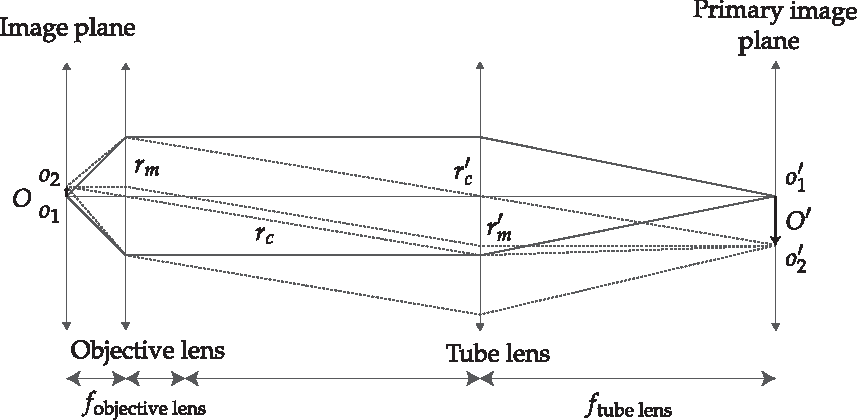
\includegraphics{./magnification}
    \caption{}
    \label{fig:magnification}
\end{figure}

% Tube lens may also be used to correct for image abberations

%Great advantage is that the lgiht path behind the objective only contains paralel light, means can add optical elements without distortions the beam path.

% Other adsvantage is you can focus by moving the objective lens

%and the overall magnification of the

%\subsubsection{Magnification}

\subsubsection{Field of view}

The observable objective field (FOV) is limited by the aperture stop of the system typified as the field number ($F_n $) and the objective lens magnification $M_{\text{object}}$:
%The maximum field of view ($F_{n}$)available is by :

\begin{align}
FOV = \frac{F_{n}}{M_{\text{object}}}
\end{align}

The field number of objective lenses is limited by the image degradation caused by optical aberrations, with modern objective technology reaching up to \SI{28}{\milli\meter} from the previous standard of \SI{20}{\milli\meter}.

\subsubsection{Illumination}

The illumination system defines the contrast mode, the resolution of the instrument, and the overall brightness.
Two principally different optical setups are in use.
The simpler one is the source focus or critical illumination and the other, which is by far more prevalent, is called Köhler illumination.

Critical illumination uses a single \emph{condenser} lens whereas Kohler illumination uses a \emph{collector} lens as well.
The use of two illumination lenses allows for a conjugate 4f system of illumination to the detection optics, this ensures that all ray bundles passing through the sample are parallel and the illumination brightness is homogenous.
Having a conjugated illumination also allows for alternative contrast methods to be implemented. %TODO sort

In the illumination beam paths discussed earlier, the specimen is placed between the light source and the objective lens.
In many cases, however, it is advantageous to illuminate the specimen from the side of observation (\emph{epi-illumnination}), for instance, when looking at the reflection of opaque or fluorescent samples.
In that case, some optical components of illumination and imaging are identical, for example, the objective lens. %TODO reword


\subsection{Resolution}

%Magification versus resolution

Resolution refers to the level of detail that can be recognized in an image, such as small and intricate structures or the distance between closely placed small objects.
Indeed, such a distance is used to define and quantify the optical resolution.
Using light microscopy, minute objects can be discriminated from each other when they are positioned at a minimum distance of -0.25 mum from each other and green light and a high-quality oil-immersion objective lens are used.
This obviously means that proteins and supramolecular complexes occurring in living cells cannot be recognized in detail.
In later chapters, we discuss how the principal optical resolution limit can be overcome or circumvented by advanced optical techniques.

%Bragg conditions
%

\begin{align}
    d \sin \alpha_n = n \lambda \\
    \sin\alpha_n = \frac{p_n}{f} \\
    p_n = \frac{n\lambda f}{d} \\
    d \le = \frac{\lambda}{\sin\alpha_{\text{max}}} \\
    d \le = \frac{\lambda_0}{n\sin\alpha_{\text{max}}} = \frac{2\lambda_0}{NA}
\end{align}

\subsubsection{Angular and numerical aperture}

%An objective lenses is limited by
The maximum acceptance angle ($\alpha$) of an objective lens limits the amount of light that can be collected from the sample.
An objective lens at the may be approximated to applying a Fourier transform of the imaging space, through an aperture with radius $a$ with an imaging plane at the far field.
This leads to high frequency information being omitted during the imaging process and the microscope behaving as a low-pass filter.
The electric field ($E(r)$) and resultant intensity ($I(r)$) distribution of a single point (delta function) at the image plane then becomes:

\begin{align}
    E(r) &\propto E_0 \frac{J_1 \left(2\pi r \sin \frac{\alpha}{\lambda}\right)}{2\pi r \sin \frac{\beta}{\lambda})}\label{eq:E_airy}\\
    \implies
    I(r) &= I_0 \left[\frac{J_1 \left(2\pi r \sin \frac{\alpha}{\lambda}\right)}{2\pi r \sin \frac{\alpha}{\lambda})}\right]^2\label{eq:I_airy}
\end{align}

Where $J_1$ is a Bessel function of the first kind and $\beta$ is the half opening angle of the tube lens.
This function is more commonly known as as Airy disk \ref{fig:airy_disk}.

% \begin{figure*}
%     \centering
%     \begin{subfigure}
%         %\centering
%         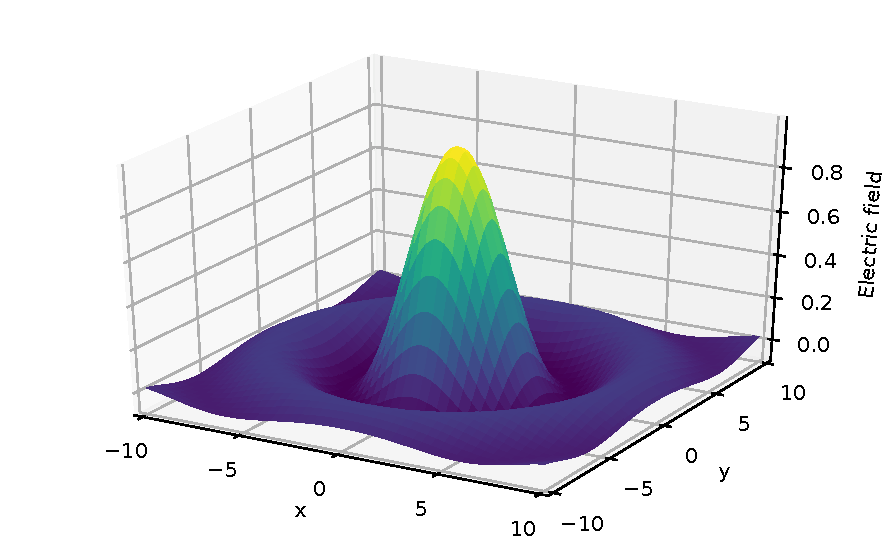
\includegraphics{airy_E_fill}
%         \caption{}
%     \end{subfigure}
%     \begin{subfigure}
%         %\centering
%         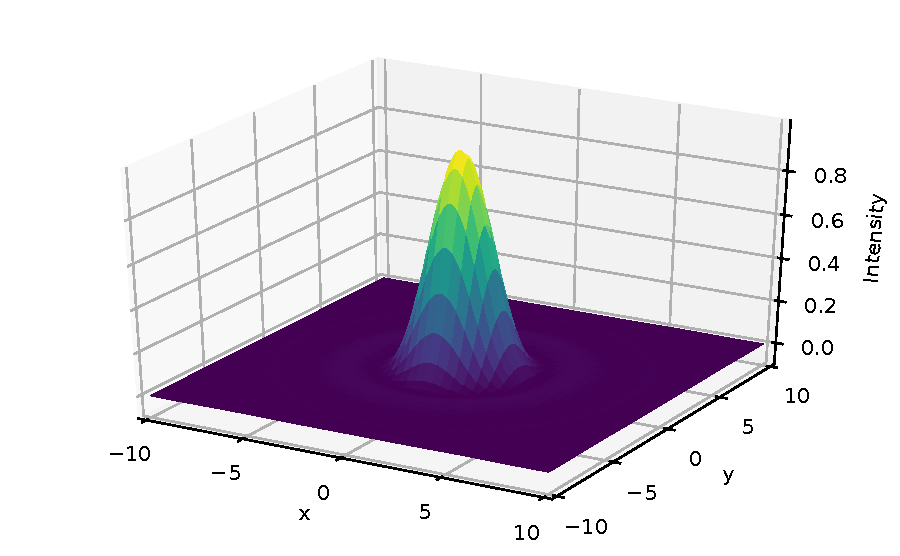
\includegraphics{airy_I_fill}
%         \caption{}
%     \end{subfigure}
%     \caption{}
%     \label{fig:airy_disk}
% \end{figure*}

\begin{figure}
    \centering
    \begin{subfigure}[b]{\textwidth}
        %\centering
        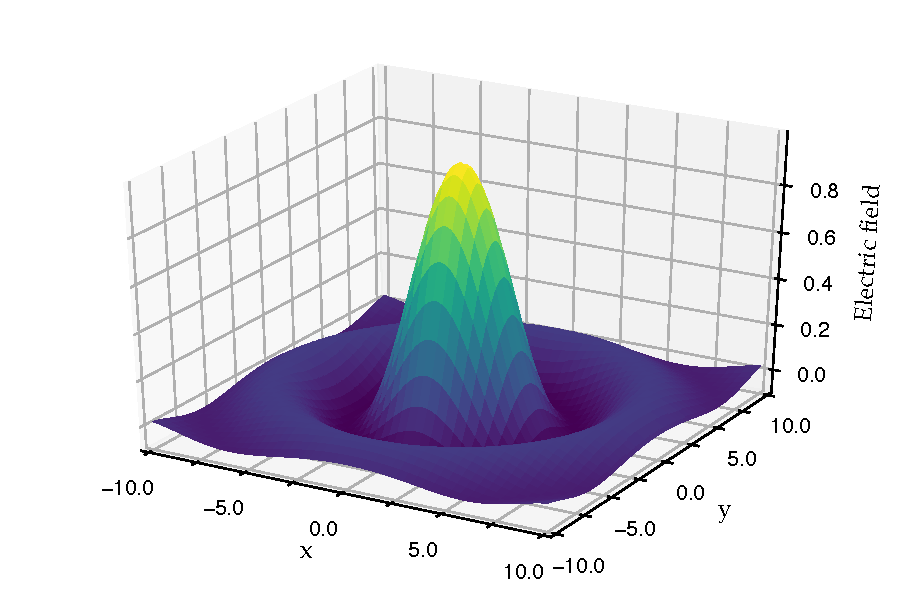
\includegraphics{+airy_E_fill}
        \caption{$E(r)$, equation \eqref{eq:E_airy}}
        \label{fig:airy_E_fill}
    \end{subfigure}
    ~
    \begin{subfigure}[b]{\textwidth}
        %\centering
        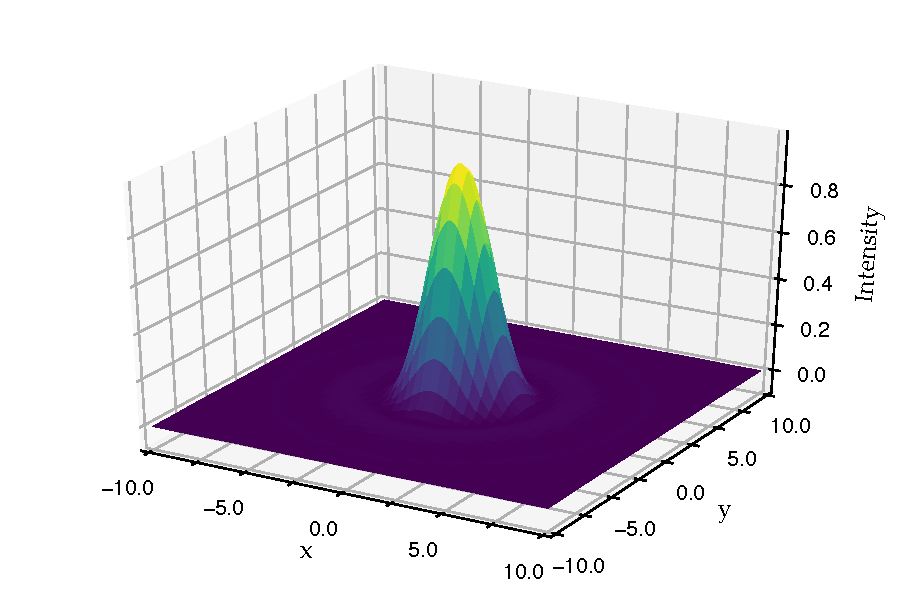
\includegraphics{+airy_I_fill}
        \caption{$I(r)$, equation \eqref{eq:I_airy}}
        \label{fig:airy_I_fill}
    \end{subfigure}
    \caption{Electric and intensity amplitudes of a theoretical airy disk in radial units of $2\pi r \sin \frac{\alpha}{\lambda}$}
    \label{fig:airy_disk}
\end{figure}

\subsubsection{Lateral resolution}

Point emitters are therefore imaged more faithfully with a wider collecting angles and with higher frequency light.
By placing two point emitters close such that the first zero crossing of the Bessel junction $J_1$ coincides with the centre of the second point emitter gives a distance of:

\begin{align}
    r_0,\text{objective} &\approx \frac{0.61\lambda}{n\sin\alpha} = d_r \\
    \implies d_r &= \frac{1.22 \lambda}{NA_{\text{objective}}}
\end{align}

The resulting distance is Rayleigh's criterion for resolution which provides a limit to the resolution of a system based on a dip in intensity maxima, between two neighbouring emitters, of $\sim 75\%$.

%Coherent and incoherent
\subsubsection{Axial resolution}

The Airy Disk describes the in-plane of lateral intensity distribution, with an analogous analytical function propagating axially.
Once again, by comparing the the distance to the first zero in intensity along $z$ an analytical definition can be formed:

\begin{align}
    z_0,\text{objective} = \frac{2n\lambda}{NA^2} \label{eq:}
\end{align}

The achievable axial resolution is governed by axial extension of the PSF as is $2z_0,\text{objective}$ and commonly called the \emph{depth of field} ($D\text{objective}$).
The depth of field physically refers to the distance a focussed object may be moved axially before losing image fidelity to defocus.


\begin{figure}
    \centering
    \begin{subfigure}[b]{\textwidth}
        %\centering
        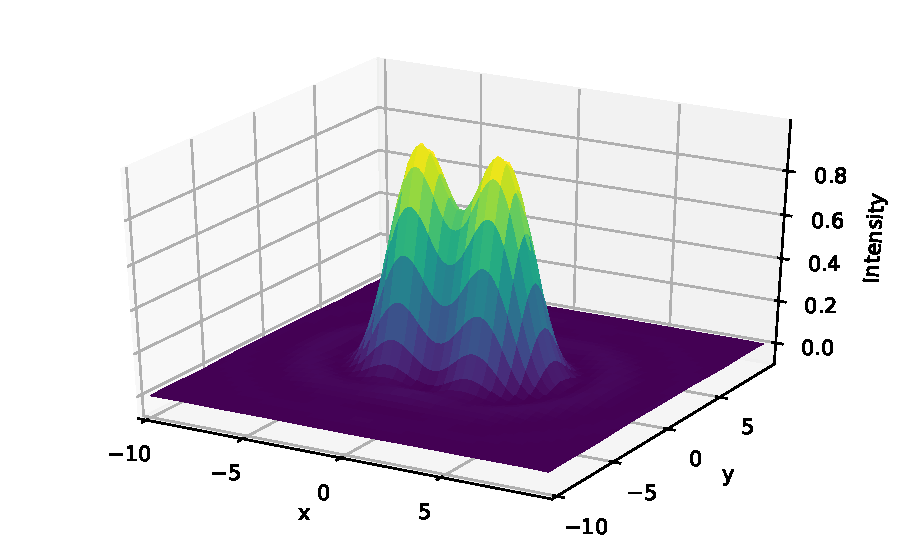
\includegraphics{+airy_rayleigh}
        \caption{The Rayleigh criteon, whereby the centre of the second emitter sits at the first zero of the first emitter}
        \label{fig:airy_rayleigh}
    \end{subfigure}
    \begin{subfigure}[b]{\textwidth}
        %\centering
        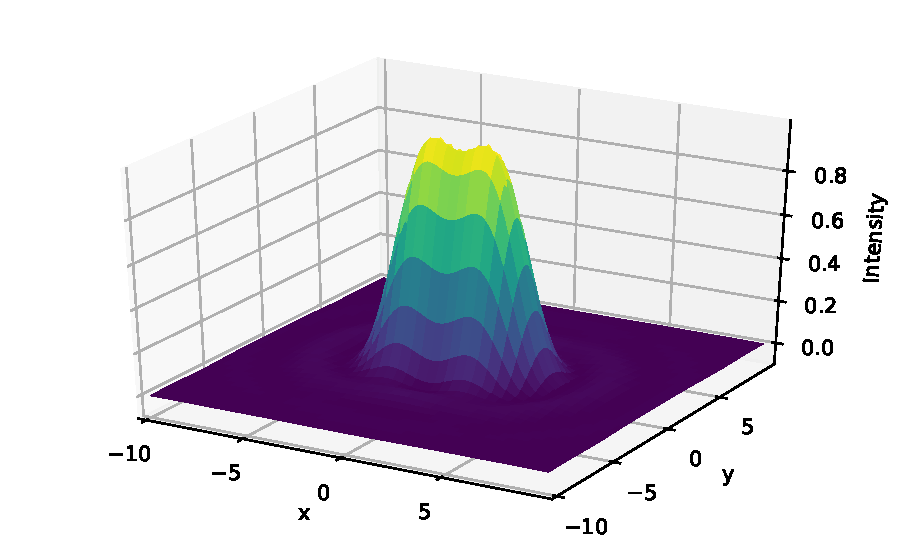
\includegraphics{+airy_sparrow}
        \caption{The Sparrow criteon, whereby the centre of the second emitter is one FWHM of the function distant from the first emitter}
        \label{fig:airy_sparrow}
    \end{subfigure}
    \end{figure}
    \begin{figure}
    \ContinuedFloat
    \begin{subfigure}[b]{\textwidth}
        %\centering
        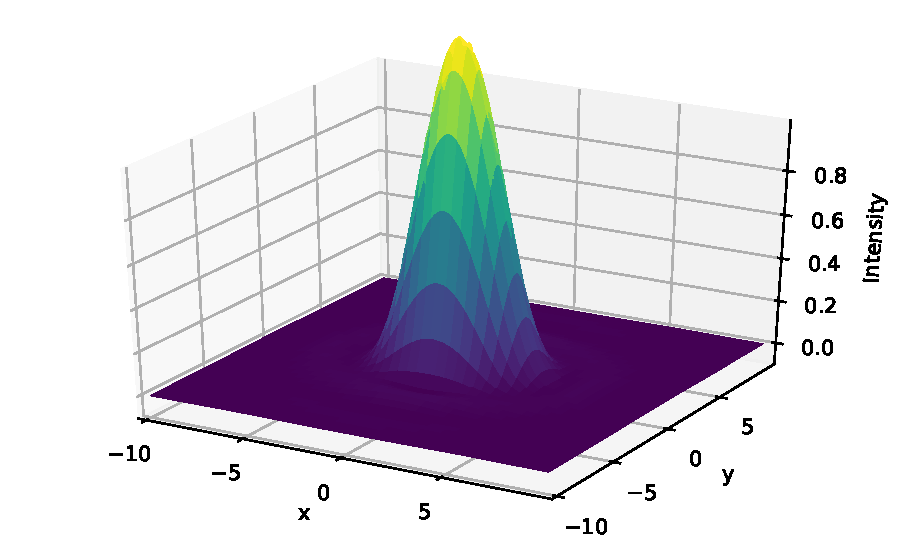
\includegraphics{+airy_too_close}
        \caption{Unresolved, depicted here as being half the Sparrow limit}
        \label{fig:airy_too_close}
    \end{subfigure}
    \caption{The resolution of a system is governed by the resolving capability of two nearby point emitters.
    (\subref{fig:airy_rayleigh}) and (\subref{fig:airy_sparrow}) show the Rayleigh and Sparrow criterions respectively with (\subref{fig:airy_too_close}) showing point emitters too near to be resolved due to the lack of any intensity contrast between them}
    \label{fig:airy_disk_resolution}
\end{figure}

%
% Depth of field
%
% \subsubsection{Depth of field}


\subsubsection{Sampling}

Once transmitted, image information is typically recorded digitally using using a CCD camera or similar device.
According to Nyquist sampling theory the resolution of the detector required to resample the image information faithfully is $d_\text{detector} = \frac{d_r}{2}$.
To then choose the correct system magnification ($M_\text{system}$) it follows that:

\begin{align}
    M_\text{system} = \frac{2d_\text{detector}}{d_r}
\end{align}

For a detector with \SI{6}{\micro\meter} pixels a magnification on the order of $50\times$ is therefore sufficient for diffraction limited imaging using visible light.
Magnifications in excessive of this limit are deemed \emph{empty magnification} and decrease the overall SNR of the recorded image.

Over-sampling plays an important role in super-resolved systems where the additional pixel information, though diffraction limited may be used computationally to increase resolution.

\begin{figure}
    \centering
    \begin{subfigure}[b]{\textwidth}
        \centering
        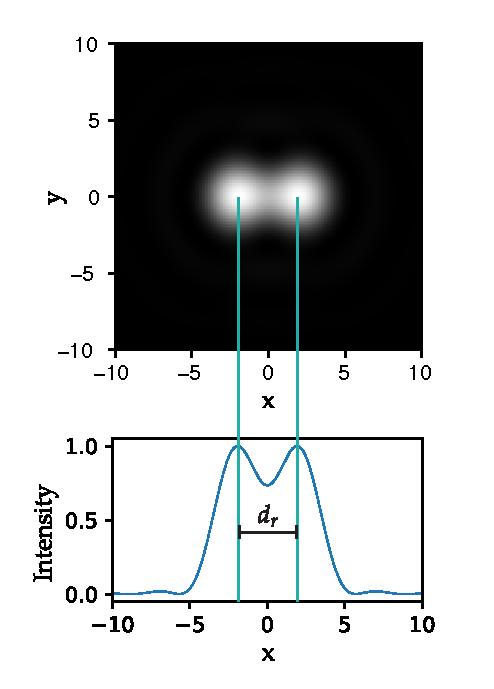
\includegraphics{./sampling/sample_master}
        \caption{Intensity image of a pair of resolved point emitters separated by the Rayleigh distance $d_{r}$}
        \label{fig:sample_master}
    \end{subfigure}
\end{figure}~
\begin{figure}
    \ContinuedFloat
    \centering
    \begin{subfigure}[b]{0.4\textwidth}
        \centering
        
\includegraphics[width=0.9\textwidth]{./sampling/digital_airy_sample_3}
        \caption{Sampled using 3 by 3 pixels\\$d_{\text{detector}} = 1.5 \times  d_{r}M_{\text{system}}$}
        \label{fig:digital_airy_sample_3}
    \end{subfigure}~
    \begin{subfigure}[b]{0.4\textwidth}
        \centering
        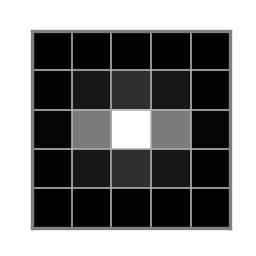
\includegraphics[width=0.9\textwidth]{./sampling/digital_airy_sample_5}
        \caption{Sampled using 5 by 5 pixels\\$d_{\text{detector}} = 0.9 \times  d_{r}M_{\text{system}}$}
        \label{fig:digital_airy_sample_5}
    \end{subfigure}
    \begin{subfigure}[b]{0.4\textwidth}
        \centering
        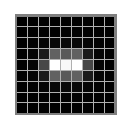
\includegraphics[width=0.9\textwidth]{./sampling/digital_airy_sample_9}
        \caption{Sampled using 9 by 9 pixels\\$d_{\text{detector}} = 0.5 \times d_{r}M_{\text{system}}$}
        \label{fig:digital_airy_sample_9}
    \end{subfigure}~
    \begin{subfigure}[b]{0.4\textwidth}
        \centering
        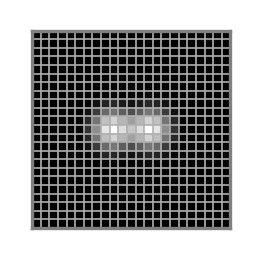
\includegraphics[width=0.9\textwidth]{./sampling/digital_airy_sample_23}
        \caption{Sampled using 23 by 23 pixels\\$d_{\text{detector}} = 0.19 \times d_{r}M_{\text{system}}$}
        \label{fig:digital_airy_sample_23}
    \end{subfigure}
    \caption{Point emitters in \subref{fig:sample_master} are sampled by a detector varying pixel sizes, analogous to varying magnification.
    (\subref{fig:digital_airy_sample_9}), shows Nyquist sampling;
    (\subref{fig:digital_airy_sample_23}) is over sampled, giving super detector resolution
    (\subref{fig:digital_airy_sample_3}) and (\subref{fig:digital_airy_sample_5}) do not preserve resolution as they are below Nyquist sampling and hence detect a single emitter.}
    \label{fig:airy_disk_resolution}
\end{figure}


%
% \subsubsection{Light collection efficiency}
%
% To calculate the the collecting efficiency of a lens, a single radiating source is considered, a Lambert radiator.
% The flux collected is proportional to the spherical segment carved out by the lens.


\section{Fluoresence microscopy}
\subsection{Contrast in optical microscopy}
% Phase contrast, dark field
\subsection{Fluoresence}

Fluorescent molecules absorb photons of a particular energy and a short time later remit them with lower energy, this energy difference gives rise to a red-shift of the light.
This shift in colour allows for suitably coated glads to chromatically discriminate between the desired fluoresecent signal and the undesired scattered incident light.
Upon being exciting by incident light an electron within a fluorescent molecule may excite to a higher energy level, provided it has sufficient energy to bridge the energy barrier.
Once in the higher excited state ($S_1$), the electron will exist there for an average lifetime ($\tau$), slowly losing energy to the surroundings through vibrations and molecular collisions.
Once the electron has ''trickled'' down the energy levels it will return to the ground state ($S_0$) emitting a photon with an energy less the amount of energy lost when in the excited state, the \emph{Stoke's shift}.
Electrons may also return to the ground state through molecular collisions or even an \emph{intersystem} crossing where by the electron finds a path via transient state with lower energy requirements, the \emph{triplet state}.

%\subsubsection{Fluoresence spectra}

Multiple energy levels slightly above the ground state and the excited states then allow multiple different emission wavelengths.
Fluorescent molecules therefore have excitation and emission spectra rather than discrete excitation and emission lines, see Figure \ref{fig:fluo_spectra} for typical fluorescent molecules used in microscopy.

\begin{figure}
    \centering
    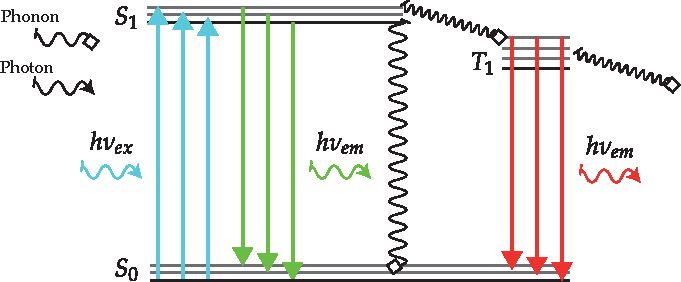
\includegraphics[width=0.7\linewidth]{jablonski_triplet_new}
    \caption[Standard jablonski diagram]{Jablonski diagram representing in colour the excitation of Alexa Fluor\(^{\copyright}\) 488 in a standard two level fluorescent system.}\label{fig:jablonski_triplet_new}
\end{figure}

%\subsubsection{Specificity}

\emph{Specificity} refers to the ability to accurately label markers, features or molecules within a biological entity and is an important advantage of fluorescence microscopy.
Moreover multiple labels can further elucidate how labelled entities are interact within the the sample.

\subsubsection{Labelling}


Labelling of sites direct, primary and secondary.
Resolution is lost the longer the ligand attaching to the target but for convenience of dyes with the suitable anti-group being available.
The staining process is further inhibited by cellular mechanics; a cell may not endocytose the stain or be it may degraded through autophagy in the lysosome.
For non-membrane permeable dyes transfection techniques, though invasive, do exist \cite{}.
Staining can also lead to non-specific binding of fluorescent molecules reducing confidence in specificity and increasing the overall background fluorescent signal in-turn decreasing the image contrast.

For live organism imaging, staining is impractical.
Genetic manipulation causes fluorescent proteins to be expressed with high specificity as
As the cells themselves are producing the desired fluorescence; with good spatial homogeneity when compared to soaking samples in dye; and low sample toxicity.


\begin{figure}
    \centering
    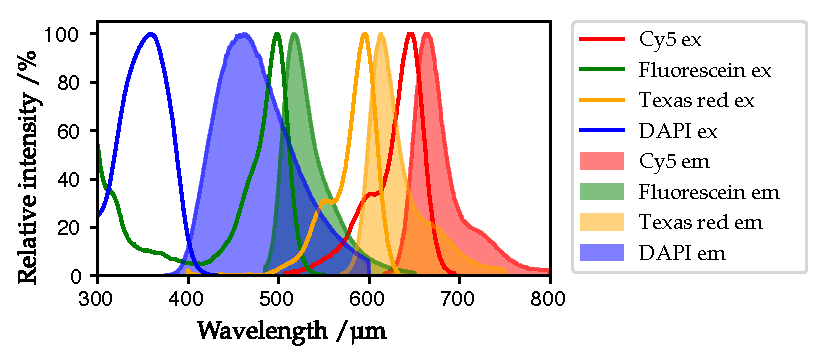
\includegraphics{./fluorphores/++multi_plot.pdf}
    \caption{Fluorescence excitation (lines) and emission (filled curves) spectra of the compounds Fluorescein, Texas red, Cy5 and DAPI.}
    \label{fig:fluo_spectra}
\end{figure}
%TODO Talk about auto Fluoresence

%\subsubsection{Image contrast}
%\subsubsection{Specificity}
\subsection{Fluoresence microscopy}

\subsubsection{Illumnination}

%The Merucry Arc lamp is unibiqitous in lamp-based fluorsence mciroscopes.
The mercury arc lamp became a ubiquitous excitation source due an visible emission spectrum and intensity being much greater than a standard halogen lamp.
However, advances in LED and laser technology have caused a technological shift towards these alternative sources.
Modern LEDs and Lasers are now at the stability and intensity to compete with lamp based sources, with more intensity ability and homogeneity.

LED sources are currently behind Lasers in terms of the intensity required for certain imaging applications due to the \emph{etendue} of the emission.
As etendue is preserved through any system of optics an LED source, having large etendue, will be very photon inefficient to the point of being infeasible for applications such as point-scanning.

Lasers are limited to very specific excitation lines due to the materials used, particular in diode lasers.
These sources are also coherent which can cause self-interference in the illumination profile (speckle) and the sample.
%For wide-field imaging LED sources may be sufficient with an added benefit of being incoherent.

%Emission wavelengths are selected from lamp and white LED sources using emission filters.
A super-continuum laser sources uses non-linear effects, typically induced within a long optical fibre , to produce broad spectrum visible laser light.
From this spectrum, wavelengths may then be selected using emission filters, as with lamp-based sources and white LED sources.
To add additional emission lines into a system with monochromatic lasers requires adding more laser lines physically, this approach is desirable for making systems versatile.
The downside being that the intensity of the of the pump laser source is spread into the entire spectrum causing narrow selected emission bands to have relatively low intensities.


\subsection{Signal collection}

Once created, the sample image is recorded for analysis and dissemination.
%Modern camera technology
For contemporary digital pixel (photosite) arrays are used in wide-field fluoresce microscope where as photo-multiplier tube (PMT) in \emph{most} laser scanning microscopy.

\subsubsection{Detectors}

Wide-field detectors come in many flavours, all of which exploit semi-conductor physics to convert incident photons into electrons.
Charge-couple device (CCD) based detectors collect electrons during an exposure and transfer in a serial manner through conversion electronics to create digital images.
Intensified CDD (ICCD) follow the same protocol but use on-photo-site electron cascading to increase the signal and \emph{intensify} the read image.
EMCCD detectors transfer their entire frame to a separate conjugate chip which digitises the image for computation.
As the frame is being transferred the signal is amplified to multiply electrons collected in the conjugate digitisation site and intensify the image as in ICDD.
Transferring the entire frame reduces the digitalisation time and increase the imaging frame-rate.

CMOS chips directly output a digital value on a per pixel.
The additional circuity found off-chip in CCD detectors is embedded in each pixel.
Though this reduces the overall fill factor feasible in each chip, this is recovered using a micro-lens to focus directly onto the active read area of the photo-site.
The per-photo-site architecture allows for a region-of-interest area to be addressed.
CMOS detectors made specifically to address quantitative scientific (sCMOS) usage boast having: small pixel sizes; low read noise; large detection arrays; large dynamic range and no multiplicative noise.

%sCMOS

%\subsubsection{Single molecule detection}


\subsubsection{Noise}

Adverse noise arising in optical microscopes from several compounding effects.
The larger the noise level the lower the signal to noise ratio and therefore the more degraded an image will be.

Increasing the integration time of the detector will bring the desired signal out of random background noise.
A detector with a large \emph{quantum efficiency}, (photon to electron conversion efficiency) will be able to overcome noise more quickly.
The \emph{dynamic range} of the detector is the intensity range at which the weak fluorescent signal can be recorded above background noise.
The \emph{bit depth} (8 or \SI{16}{\bit} typically) of the detector defines the detectable intensity resolution, which is particular use for very weak signals.

The \emph{dark current} (noise) contribution occurs in the detectors themselves as the semiconductor material produces erroneous electrons from converting thermal phonons.
Dark current increases linearly with integration time and so chip cooling is recommended. \emph{Photon noise} (shot) originates from corpuscular photons arriving at the detector following a temporal Poissonian distribution.
An image containing $n$ photons will suffer a variation of $\sqrt{n}$ in photons being emitted, this can appear as valid structure once recorded. \emph{Read noise} is rooted in the conversion process of the analogue voltage of electrons, at each pixel, to digital values.
The intensity response across a detector may also be inhomogeneous, this may be flat-field corrected using a calibration uniform intensity source.
\footnote{manufacturers for sCMOS cameras apply this correction as standard}

\subsection{Limits of fluorescence microscopy}


\subsubsection{Photobleaching}

Fluorescently stained samples will slowly fade in intensity over time as the dye molecules are photochemically destroyed through photobleaching.
The process occurs typically through photo-oxidation, once the fluorophore is in an excited state it may then energetically fall into a triplet state where it is more likely to permanently bond with oxygen radicals.
Dye medium can be buffered with scavengers of Oxygen radicals to mitigate the process of bleaching.
Genetically modified organisms suffer from the photobleaching less as molecules that have bleached are constantly being replaced by newly expressed fluorophore.

Photobleaching can be exploited using FRAP whereby an imaging region is purposefully bleached so that dye molecules may diffuse into the field of view.
The rate of return of intensity in the imaging region then gives a measure of diffusion.

% FRET STORM PALM
%Some molecules have the valuable property of being able to reverse


%\paragraph{Reversible photobleaching}
\subsubsection{Phototoxicity}

Fluorescent dyes can act as photo-sensitizer during imaging, causing damage to functionality of the cell.
Chromophores of fluorescent proteins are shielded by direct contact from molecular oxygen through protein moiety, making fluorescent proteins less photo-toxic.
% It has beeen suggested that acceptable levels of light exposure will be on the order of a solar.
%Direct and intense light exposure
%TODO


%Photodynamic effwect
%Intensity induced
%\subsection{Resolution}
\section{Three dimensional fluorescence microscopy}
\subsection{Confocal Microscopy}

The Marvin Minksy proposed the first confocal microscope in the late 1950s to image deep into brain tissue.
A pinhole is placed in a conjugate image plane in the detection path which precludes out-of-focus light from being detected.
The narrower the pinhole the better the optical sectioning, though sacrificing the received signal.

In Minky's microscope the sample was then mechanically scanned to build a volumetric image.
By mechanically scanning the imaging speed is greatly reduced but to the speed of responses of the stage, the maximum speed of travel of the stage and the relaxation time of the stage.
Specimens are prone to spatial shifts during scanning as well which causes distortions in the final image.

Modern confocal microscopes use galvanometric scanning mirrors to scan a laser beam through the sample to build an image.
Though faster than mechanical scanning, video-rate scanning confocal microscopy is only viable when using resonant scanning mirrors and high laser power.

% \subsubsection{Spinning disk confocal microscopy}
%
% The speed of Single point confocal microscopy can be greatly improved by producing multiple points.

%\subsubsection{Principles}
%\paragraph{Spinning disk confocal microscopy}
\subsection{Two photon (2P) microscopy}

% 2P microscopy is a part of a breed of techniques called non-linear microscopes which exploit the quantum nature of fluorophores.
% 2P imaging provides the most efficient signal generation.

The photon rejecting pin-hole of confocal microscopes can be entirely avoided by using infra-red laser sources.
Exciting a fluorophore to an excited state requires a quantised amount of energy, which is typically supplied by a single photon.
Two photons, each with double the desired wavelength, will contain the requisite amount of energy to cause the excitation.
For this event to occur there need to be a high photon density surrounding the fluorophore.
In a laser scanning system, this means that the beam focus of the objective lens is the most likely place for fluorescence to occur, with a sharp decline in axial intensity axially, providing optical sectioning.

By using 2P excitation greater depth imaging (\SI{\sim6}{fold} deeper) can be achieved with reduced photo-toxicity, making the technique very useful for non-invasive live imaging.

\subsubsection{Drawbacks}

Water, which is abundant in biological specimens, has large absorbance in the infrared spectrum; combined with the high energy needed to create the 2P effect at the focal point, this can cause localised heating which can in-turn be damaging to specimens and cause optical aberrations.
Localised heating can be mitigated by moving the beam sufficiently quickly such that significant heating does not occur.
Using infrared excitation also means that the 2PM has a much reduced theoretical lateral resolution when compared to visible confocal microscopy.
Finally, infrared-red laser sources are prohibitively expensive and, until recently, reliable turn-key solutions were not viable.

\subsection{Structured illumination microscopy}

In SIM, a specimen is illuminated with a sinusoidal periodic pattern using a fast widefield microscope.
The mixing of this illumination frequency with the spatial frequency of the sample means that additional resolution can be extracted both in $xy$ and $z$.

As discussed, an objective lens acts as a band pass filter for low-frequency information.
From the \emph{Convolution Theorem} (see Appendix \ref{appendix:convolution_theorem}), the multiplication of two signals in real-space is the convolution of the two Fourier transformed signals in frequency space and, importantly, visa versa -
the convolution of two signals in real space is the multiplication of the Fourier transformed signals in frequency space.
Meaning that projecting a sinusoidal pattern in real space will convolve the Fourier transform of the sample signal in frequency space with the Fourier transform of the sinusoid signal.
The Fourier transform of a sinusoid is three delta functions at -1 0 and +1 with a separation governed by the pattern frequency: $k_1 = {2\pi}{lambda}$.
And so, before the imaging system can band-pass the signal, the illumination pattern has forced three copies of the original image into the pass band, shifted by the vectors $k_1$ and $k_{-1}$ such that high frequency information outside of the pass band has been cumulated.
The overlaid information is then computational unmixed by imaging with three different sinusoid phases to delineate the \SI{-1}{} \SI{0}{} and \SI{+1}{} orders or reconstruction.

\subsubsection{Optical sectioning SIM}

Three dimensional information can be extracted by manipulating frequency space even further.
For instance, the \emph{missing cone} (see Figure \ref{fig:OTF_support}) can be filled in by using an illumination pattern with $k$-vectors half the maximum available.
In frequency space this pushes the region of the missing cone into axial resolution maxima of the OTF support (toridal), giving three dimensional structure.
By adding a third beam along the optical axis to interfere with the sinusoidal pattern, a further axial sinusoidal pattern can be created.

\subsubsection{Drawbacks}


\subsection{Selective plane illumination microscopy}

The technqiues for volumetric imaging as introduced above

Structured illumination techniques require computation reconstruction which is prone to artefacts.

Light-sheet microscopy offers reconstruction free (SIM), fast, low photo-toxic volumetric imaging.


are limited by speed and

In light sheet microscopy, the sample is illuminated with a thin sheet of light to obtain optical sections.
The microscope generally consists of two orthogonal optical axes: one for generating the light sheet for illumination, and the other for widefield detection of the emitted fluorescence.
The two axes are aligned such that the illuminating light sheet is positioned in the focal plane of the detection unit.
As the specimen is illuminated with a sheet of light, the entire focal plane of the detection arm is illuminated providing instant optical sectioning as opposed to the slow point scanning used in confocal microscopy (Chapter 5).
